%----------------------------------------------------------------------------------------
%	PACKAGES AND OTHER DOCUMENT CONFIGURATIONS
%----------------------------------------------------------------------------------------

\documentclass[12pt]{article}
\usepackage[T5]{fontenc}
\usepackage[utf8]{inputenc}
\usepackage[vietnamese,english]{babel}
\usepackage{amsmath}
\usepackage{amsfonts}
\usepackage{graphicx}
\usepackage[colorinlistoftodos]{todonotes}
\usepackage{listings}
\usepackage{hyperref}
\usepackage[figurename=Hình]{caption}
\usepackage{algorithm}
\usepackage[noend]{algpseudocode}
\hypersetup{
    colorlinks=true,
    linkcolor=black,
    filecolor=magenta,      
    urlcolor=cyan,
    citecolor=black,
}

%----------------------------------------------------------------------------------------
%	MULTI FOOTNOTE
%----------------------------------------------------------------------------------------

\let\oldFootnote\footnote
\newcommand\nextToken\relax

\renewcommand\footnote[1]{%
    \oldFootnote{#1}\futurelet\nextToken\isFootnote}

\newcommand\isFootnote{%
    \ifx\footnote\nextToken\textsuperscript{,}\fi}
%----------------------------------------------------------------------------------------

\makeatletter
\renewcommand*{\ALG@name}{Thuật toán}
\makeatother

\addto{\captionsenglish}{\renewcommand*{\contentsname}{Mục lục}}
\addto{\captionsenglish}{\renewcommand*{\refname}{Tài liệu tham khảo}}
\renewcommand*{\thefootnote}{(\arabic{footnote})}

\captionsetup[table]{name=Bảng}
\usepackage{array}
\newcolumntype{P}[1]{>{\centering\arraybackslash}p{#1}}

\begin{document}

%----------------------------------------------------------------------------------------
%	TITLE SECTION
%----------------------------------------------------------------------------------------
\begin{titlepage}

\newcommand{\HRule}{\rule{\linewidth}{0.5mm}}

\center % Center everything on the page
 
%----------------------------------------------------------------------------------------
%	HEADING SECTIONS
%----------------------------------------------------------------------------------------

\textsc{\LARGE Đại học quốc gia TP.HCM}\\
\textsc{\LARGE Trường Đại học Khoa học tự nhiên}\\[1.5cm]

%----------------------------------------------------------------------------------------
%	LOGO SECTION
%----------------------------------------------------------------------------------------


\includegraphics{logo/rsz_3logo-khtn.png}\\[1cm] % Include a department/university logo - this will require the graphicx package

\textsc{\Large Ngành khoa học máy }\\[0.5cm]
\textsc{\large Môn học: Mã hóa ứng dụng }\\[0.5cm]

%----------------------------------------------------------------------------------------
%	TITLE SECTION
%----------------------------------------------------------------------------------------

\HRule \\[0.4cm]
{ \huge \bfseries Đồ án cá nhân}\\[0.4cm] {\huge \bfseries Cài đặt thuật toán mã hóa RSA}
\HRule \\[1.5cm]
 
%----------------------------------------------------------------------------------------
%	AUTHOR SECTION
%----------------------------------------------------------------------------------------

\begin{minipage}{0.45\textwidth}
\begin{flushleft} \large
\emph{Học viên:}\\
Đỗ Quốc Thế -- 19C11040 % Your name
\end{flushleft}
\end{minipage}
~
\begin{minipage}{0.5\textwidth}
\begin{flushright} \large
\emph{Giảng viên:} \\
PGS.TS Nguyễn Đình Thúc % Supervisor's Name
\end{flushright}
\end{minipage}\\[2cm]
%----------------------------------------------------------------------------------------

%----------------------------------------------------------------------------------------
%	DATE SECTION
%----------------------------------------------------------------------------------------
%{\selectlanguage{vietnamese}\today} \\[2cm]

\vfill % Fill the rest of the page with whitespace

\end{titlepage}

%----------------------------------------------------------------------------------------
%	TABLE OF CONTENTS SECTION
%----------------------------------------------------------------------------------------

{
  \hypersetup{linkcolor=black}
  \tableofcontents\newpage\cleardoublepage
}

%----------------------------------------------------------------------------------------
%	CONTENTS SECTION
%----------------------------------------------------------------------------------------

\section{Giới thiệu}
Đồ án cài đặt lại thuật toán mã hóa RSA với số $p$, $q$ là các số nguyên tố 1024 bits bằng ngôn ngữ lập trình C++. 
Phần cài đặt này gồm 2 quá trình chính tương ứng với 2 quá trình chính trong mã hóa RSA: 
quá trình \textit{phát sinh key} và quá trình \textit{encrytp/decrypt}.
Quá trình cài đặt sử dụng các thuật toán trong trong môn học như thuật toán nhân lấy phần dư, 
thuật toán lũy thừa lấy phần dư, thuật toán Bezout nhị phân, thuật toán số dư trung hoa và một số thuật toán khác. 

Do đã thử qua một số thư viện số nguyên lớn được \textit{public trên Github} và nhận thấy các thư viện khá chậm với số lớn và cồng kềnh nên đồ án tự cài đặt số nguyên lớn bằng các kĩ thuật lập trình căn bản.
Qua nhiều \textit{version} cải tiến, đồ án đã thực hiện được 2 quá trình chính kể trên với thời gian thực.
Báo cáo này xin được trình bày 2 cách làm tốt nhất hiện đã đạt được. 

Cách làm thứ nhất (cách 1) \textit{code} lại hoàn toàn cách xử lý với số nguyên lớn mà không dùng thư viện hỗ trợ số nguyên lớn nào, 
cách làm này lưu trữ các chữ số trong dãy \textit{bit nhị phân} dưới kiểu dữ liệu \textit{char*} cùng với các hàm thao tác nhanh nhất trong C/C++ như \textit{memcpy, memset}
và dùng các thuật toán trong chương trình học cùng với một số thuật toán tìm hiểu được từ các paper trên mạng.

Cách làm thứ hai (cách 2) cũng hoàn toàn tự \textit{code} lại các thuật toán tuy nhiên có xử dụng kiểu dữ liệu nhiều bit hơn các kiểu dữ liệu thông thường có trong C++, 
cách này định nghĩa lại một kiểu số 4096 bits bằng thư viện Boost Multiprecision\footnote{https://t.ly/CmsG}.

Cách làm thứ nhất thời gian thực thi các phép toán là không chậm nhưng cách làm thứ hai tối ưu hơn và đạt được thời gian xử lý rất nhanh. 
Kết quả chính của đồ án này là từ việc cài đặt theo cách 2. Tuy nhiên báo cáo cũng có sự so sánh giữa 2 cách cài đặt để rút ra được kết luận cuối cùng. Các phần tiếp theo trong 
báo cào sẽ nói về những bước cài đặt của đồ án, ở mỗi bước, báo cáo sẽ nói về cài đặt theo mỗi cách đã nêu ở trên.

Tuy đã cố gắng rất nhiều nhưng đồ án không tránh khỏi những thiếu sót nhất định, mong nhận được sự đóng góp của thầy để hoàn thiện hơn về kĩ năng và kiến thức 
cho những lần báo cáo tiếp theo. Cảm ơn thầy!\newpage\cleardoublepage

\section{Cài đặt tính toán cơ bản}
\subsection{Số nguyên lớn}
Bước này là bước rất quan trọng hơn cả vì không cài đặt được cách lưu trữ số nguyên lớn thì không thể thực hiện các bước tiếp theo. Cài đặt số nguyên lớn chỉ phức tạp khi thực hiện theo cách 1.

 Trong cách làm 1, các số được lưu dưới dạng dãy bit nhị phân, mỗi dãy bit là một con trỏ \textit{char*} 
và overload lại các toán tử cần dùng cho chương trình như \textit{+; $-$; $\%$; $\gg$,  $\ll$, >, ==, >=}. Mỗi lần thực hiện các phép toán làm 
thay đổi độ dài của chuỗi bit nhị phân thì cần tạo lại vùng nhớ mới nên đồ án dùng các hàm có tốc độ xử lý cao như \textit{memset}, \textit{memcpy}.

Đối với cách làm 2, chỉ cần dùng thư viện Boost khai báo kiểu số 4096 bit như code dưới dây:

\begin{center}
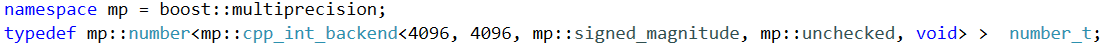
\includegraphics[width=1\textwidth]{image/number_t.PNG}
\end{center}

Như vậy ta có thể sử dụng kiểu dữ liệu mới là \textbf{number\_t} với các phép toán built-in như đối với các phép toán trên số nguyên trong C++. Điều này giúp cải thiện rất nhiều chi phí tính toán.

\subsection{Phép Mod}
Phần phép tính quan trọng tiếp theo sau khi đã tìm được các biểu diễn số nguyên lớn là cài đặt phép toán modulo. Nếu dùng kiểu dữ liệu \textbf{number\_t} 
như phần trước trình bày thì phần này không có gì đặc biệt vì chỉ cần dùng phép toán $\%$ của kiểu dữ liệu. Nếu cài đặt lại kiểu dữ liệu số nguyên lớn thì phần này cực kì quan trọng vì tất cả các bước xử lý trong các bước tiếp theo đều dùng tới phép modulo.

Thực nghiệm cho thấy cách tính modulo truyền thống như \textit{Thuật toán \ref{alg:mod}} khi tính cho số nguyên lớn rất chậm, 
đồ án đã cài đặt thuật toán modulo theo bài báo \cite{Will14computingmod}, nội dung của thuật toán này thể hiện trong  \textit{Hình \ref{fig:modwithoutmod}}.

Với việc cài đặt thuật tóan modulo cải tiến, tốc độ chương trình được cải thiện rất nhiều.
\newpage
\begin{algorithm}
\caption{Thuật toán modulo}\label{alg:mod}
\hspace*{\algorithmicindent} \textbf{Input:} BigInt a, BigInt b\\
\hspace*{\algorithmicindent} \textbf{Output:} a \% b
\begin{algorithmic}[1]
\Procedure{Mod}{$a,b$}
\While{$a > b$}
\State $a\gets a - b$
\EndWhile\label{euclidendwhile}
\State \textbf{return} $a = b $ ? 0 : $a$
\EndProcedure
\end{algorithmic}
\end{algorithm}

\begin{figure}[!h]
    \centering
    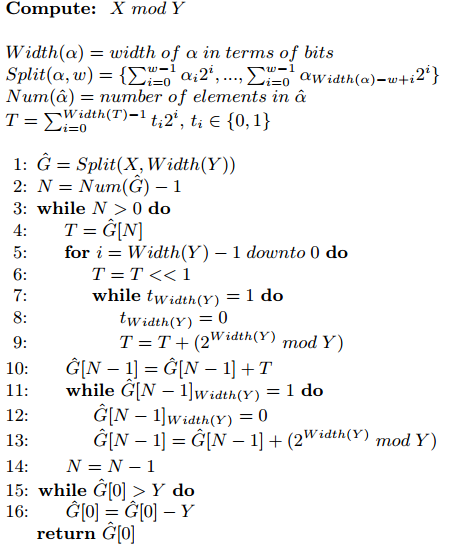
\includegraphics[width=1\textwidth]{image/mod_without_mod.PNG}
	\centering
	\caption{\label{fig:modwithoutmod} Thuật toán tính nhanh Mod trong \cite{Will14computingmod}}
\end{figure}




\subsection{Phép MulMod}
Cũng như việc cài đặt phép tính \%, việc cài đặt phép tính MulMod dùng kiểu dữ liệu \textbf{number\_t} đã định nghĩa không có gì đặc biệt ngoài việc đảm bảo 
không bị tràn số, tuy nhiên với kiểu dữ liệu 4096 bits thì việc tràn số trong phép nhân với hai số 1024 bits không thể xảy ra vì phép nhân số $n$ bits và số $t$ bits 
cho ra kết quả nhiều nhất là $n + t + 2$ bits (\textit{\cite{Menezes} Chương 14 trang 595}). Thực hiện phép MulMod với kiểu dữ liệu \textbf{number\_t} là thực hiện phép nhân 
trước rồi phép modulo sau.

Còn với cách 1, cài đặt thuật toán MulMod cho kiểu số nguyên lớn tự định nghĩa được thực hiện theo \textit{Thuật toán \ref{alg:mul-mod}} (tham khảo giáo trình).

\begin{algorithm}
\caption{Tính MulMod}\label{alg:mul-mod}
\hspace*{\algorithmicindent} \textbf{Input:} BigInt x, BigInt y, BigInt n\\
\hspace*{\algorithmicindent} \textbf{Output:} x*y\ \%\ n
\begin{algorithmic}[1]
\Procedure{MulMod}{$x,y,n$}
\State $p \gets 0$
\If {$y_0 = 1$} \Comment Bit cuối của y là 1
\State $p \gets x$
\EndIf
\For {$i \gets 1$, m}\Comment m là số bit của y
\State $x \gets 2*x\ \%\ n$ \Comment x L-Shift 1 bit rồi \% n
\If {$y_i = 1$}
\State $p \gets (p+x)\ \%\ n$
\EndIf
\EndFor
\State \textbf{Return } $p$
\EndProcedure
\end{algorithmic}
\end{algorithm}

\subsection{Phép PowerMod}
Quá trình cài đặt phép PowerMod cần thiết cho cả hai cách làm vì nếu dùng \textbf{number\_t} thực hiện phép lũy thừa thì có thể sẽ xảy ra tràn số. 
Phép toán PowerMod được cài đặt theo \textit{Thuật toán \ref{alg:power-mod}}

\begin{algorithm}
\caption{Thuật toán PowerMod}\label{alg:power-mod}
\hspace*{\algorithmicindent} \textbf{Input:} BigInt a, BigInt p, BigInt n\\
\hspace*{\algorithmicindent} \textbf{Output:} $a^p\  \% \ n$ 
\begin{algorithmic}[1]
\Procedure{PowerMod}{$a,p,n$}
\State $y \gets 1$
\If {$p = 0$}
\State \textbf{Return} \ $y$
\EndIf
\State $A \gets x$
\If {$p_0 = 1$}
\State $y \gets x$
\EndIf
\For {$i \gets 1$, m}
\State $A \gets A^2\ mod\ n$
\If {$p_i = 1$}
\State $y \gets A*y \ mod \ n$
\EndIf
\EndFor
\State \textbf{Return } $y$
\EndProcedure
\end{algorithmic}
\end{algorithm}

\subsection{Kiểm tra số nguyên tố}
Đồ án dùng định lý Fermat nhỏ để kiểm tra số số giả nguyên tố mạnh với 4 cơ sở là bốn số tự nhiên. \textit{Thuật toán \ref{alg:is-prime}} mô tả cách kiểm tra số nguyên 
tố.

\begin{algorithm}
\caption{Thuật toán PowerMod}\label{alg:is-prime}
\hspace*{\algorithmicindent} \textbf{Input:} BigInt n\\
\hspace*{\algorithmicindent} \textbf{Output:} True: là số nguyên tố, False: ngược lại 
\begin{algorithmic}[1]
\Procedure{IsPrime}{$n$}
\For {$i$\ \textbf{in}\ $\{2, 5, 7, 9\}$}
\If {$i^{n-1}\ \% \ n \neq 1$}
\State \textbf{Return } false
\EndIf
\EndFor
\State \textbf{Return } true
\EndProcedure
\end{algorithmic}
\end{algorithm}
\cleardoublepage
\section{Cài đặt tính toán cho RSA}
\subsection{Phát sinh số nguyên tố mạnh}
Việc phát sinh số nguyên tố $n$ bits thực hiện bằng việc chọn lựa ngẫu nhiên một số $n$ bits và kiểm thử xem số vừa phát sinh có phải là số nguyên tố hay không 
thông qua hàm \textit{ISPRIME} ở phần trên. Một đặc điểm đáng chú ý là các số nguyên tố đều có dạng chung\footnote{https://t.ly/vn5e} là  $6n \pm 1$, do đó có thể dùng đặc tính này để hạn chế số phép 
thử bằng cách chỉ thử những số có dạng $6n \pm 1$.

Phần cài đặt phát sinh số nguyên tố $n$ bits được thực hiện bằng cách phát sinh một số nguyên dương ngẫu nhiên $t$ có $n-3$ bits \textit{(vì 6 có 3 bits)} sau đó kiểm tra số 
$6n + 1$ hoặc số $6n - 1$ có phải số nguyên tố hay không, nếu một trong hai số trên là số nguyên tố thì chọn, ngược lại tăng $t$ lên 1 đơn vị và lặp lại quá trình. 
\textit{Thuật toán \ref{alg:gen-prime}} mô tả cách tạo số nguyên tố $n$ bits.

\begin{algorithm} [H]
\caption{Tạo số nguyên tố}\label{alg:gen-prime}
\hspace*{\algorithmicindent} \textbf{Input:} $n$: số bits\\
\hspace*{\algorithmicindent} \textbf{Output:} Số nguyên tố $n$ bits 
\begin{algorithmic}[1]
\Procedure{GenPrime}{$n$}
\State $t \gets GenNumber(n-3)$ \Comment Tạo số nguyên $n-3$ bits
\While{true}
\State $t \gets 6n + 1$
\If {\textit{IsPrime(t)}}
\State \textbf{Return } $t$
\EndIf
\State $t \gets 6n - 1$
\If {\textit{IsPrime(t)}}
\State \textbf{Return } $t$
\EndIf
\State $t \gets t + 1$
\EndWhile
\EndProcedure
\end{algorithmic}
\end{algorithm}

Đồ án cũng có cài đặt thuật toán tạo số \textbf{\textit{nguyên tố mạnh}} để tăng tính an toàn cho RSA. Số nguyên tố mạnh được định nghĩa\footnote{Giáo trình}:
\[ p \in \mathcal{P}: p - 1 = 2r,\ r \in \mathcal{P} \]

Để đơn giản, đồ án thực hiện phát sinh số nguyên tố mạnh được thực hiện dựa vào bài báo \cite{Rivest1978} của nhóm tác giả \textit{R. L. Rivest and 
A. Shamir and L. Adleman} năm 1978 (trang 9). Cụ thể, phát sinh một số nguyên tố $u$, sau đó tìm số nguyên tố đầu tiên trong dãy số $i*u + 1,\ i=2,4,6,...$\ \textit{Thuật toán \ref{alg:gen-strong-prime}} 
thể hiện việc phát sinh số nguyên tố mạnh.

\begin{algorithm} [H]
\caption{Phát sinh số nguyên tố mạnh}\label{alg:gen-strong-prime}
\hspace*{\algorithmicindent} \textbf{Input:} n: số bits\\
\hspace*{\algorithmicindent} \textbf{Output:} Số nguyên tố mạnh $\approx n$ bits 
\begin{algorithmic}[1]
\Procedure{GenStrongPrime}{$n$}
\State $u \gets GENPRIME(n-2)$ \Comment Tạo số nguyên tố $n-2$ bits
\State $t \gets 1$
\While{true}
\State $i \gets 2t$
\State $p \gets i*u + 1$
\If {ISPRIME(p)}
\State \textbf{Return } $p$
\EndIf
\State $t \gets t + 1$
\EndWhile
\EndProcedure
\end{algorithmic}
\end{algorithm}

Như trình bày ở trên nhóm tác giả R. L. Rivest phát triển cách phát sinh số nguyên tố mạnh (an toàn) nhằm tăng tính bảo mật cho RSA, tuy nhiên trong một bài báo sau 
này \cite{AreStrongPrimesNeedForRsa} \textit{(trang 1)} cũng của chính tác giả, tác giả có nói số nguyên tố mạnh không làm tăng tính bảo mật của RSA lên quá nhiều so với các số 
nguyên tố lớn thông thường, do đó không cần thiết phải dùng số nguyên tố mạnh trong RSA.

\subsection{Tìm số e và d}
Theo tham khảo tài liệu trên Iternet \footnote{https://t.ly/zGU9}\footnote{https://t.ly/LXCr} thì trong RSA thường chọn $e$ là các số nguyên tố nhỏ trong các số Fermat 
\footnote{https://t.ly/nieN} ($e \in \{3,5,17,257,65537\}$) 
rồi từ $e$ ta chọn $d$ sao cho $ed = 1\ mod\ \phi$.
Tuy nhiên, như trong giáo trình môn học, để an toàn hơn không nên chọn trước số $e$ nhỏ rồi chọn $d$ vì $d$ có khả năng sẽ nhỏ, nên chọn các số $d \geq \sqrt[4]{n}$.

Ở đây đồ án thực hiện chọn $e, d$ bằng cách chọn $e$ là các số nguyên tố $\geq 63357$, chọn $d$ tương ứng với mỗi $e$ được chọn sau đó kiểm tra điều kiện $d \geq \sqrt[4]{n}$ 
nếu $d$ thỏa thì chọn cặp $e, d$. \textit{Thuật toán \ref{alg:gen-ed}} minh họa quá trình tạo $e$, $d$

Thuật toán tìm $d$ khi biết $e, \phi$ được dùng là thuật toán Bezout nhị phân tham khảo từ tài liệu \cite{giaotrinh} (Phần thuật giải 1.49, trang 26).

\begin{algorithm}
\caption{Thuật toán tạo key $e$, $d$}\label{alg:gen-ed}
\hspace*{\algorithmicindent} \textbf{Input:} $p, q$: Hai số nguyên tố lớn\\
\hspace*{\algorithmicindent} \textbf{Output:} $e$, $d$ sao cho $ed = \ 1\ mod\ \phi\ ,\phi\ =\ (p\ -\ 1)(q\ -\ 1)$ 
\begin{algorithmic}[1]
\Procedure{GenKeys}{$p, q$}
\State $n \gets p*q$
\State $\phi \gets (p\ -\ 1)(q\ -\ 1)$
\State $t \gets 10922$ \Comment $6t + 5 = 65537$
\While {true}
\State $e \gets 6t + 1$
\If {\textit{ISPRIME($e$)}}
\State $d \gets BinaryBezout(e, \phi)$
\If {$d \geq \sqrt[4]{n}$}
\State \textbf{break}
\EndIf
\EndIf
\State $e \gets 6t+5$
\If {\textit{ISPRIME($e$)}}
\State $d \gets BinaryBezout(e, \phi)$
\If {$d \geq \sqrt[4]{n}$}
\State \textbf{break}
\EndIf
\EndIf
\State $t \gets t + 1$
\EndWhile
\State \textbf{Return } $e$, $d$
\EndProcedure
\end{algorithmic}
\end{algorithm}

\subsection{Giải mã nhanh dùng CRT}
Định lí số dư trung hoa có nội dung như sau: Với $n_i \in \mathcal{P}, n_i \neq n_j\ \forall i \neq j$ và $a_i \in \mathbb{N}$. Hệ phương trình sau có nghiệm 
duy nhất trong $\mathbb{Z}_{n_1n_2\hdots n_k}$
\begin{equation}\label{sequations:abs-crt}
\begin{cases}
x &= a_1\ mod\ n_1 \\
x &= a_2\ mod\ n_2 \\
& \vdots \\
x &= a_k\ mod\ n_k
\end{cases}
\end{equation}

Chứng minh của Quisquater \& Couvreur trong \cite{Quisquater1982} thể hiện việc áp dụng CRT trong RSA như sau: Với $p, q \in \mathcal{P}, p \neq q$, $\phi\ =\ (p -1)(q-1)$, 
$e,d \in \mathbb{N}, gcd(e,\phi)\ =\ 1, ed = 1\ mod\ \phi$, $n = pq$, nếu $x = c^d\ mod \ n$ thì $x$ cũng là nghiệm của hệ phương trình:

\begin{equation}\label{sequations:crt-rsa}
\begin{cases}
x &= c^{d_1}\ mod\ p \\
x &= c^{d_2}\ mod\ q
\end{cases}
\end{equation}
\begin{center}
với $d_1\ = d\ mod\ (p - 1), d_2\ =\ d\ mod\ (q - 1) $
\end{center}

Vận dụng \textit{(\ref{sequations:crt-rsa})}, quá trình \textit{decrypt} được cải thiện rõ rệt vì thay vì tính $c^d$ và modulo $n$ thì kết quả có thể tính 
được bằng các phép tính tương tự nhưng với số bit của $p, q$ nhỏ hơn nhiều so với số bit của $d, n$.

Cài đặt \textit{decrypt nhanh} là cài đặt giải hệ phương trình CRT tổng quát \textit{(\ref{sequations:abs-crt})} từ đó giải \textit{(\ref{sequations:crt-rsa})}. 

Cho trước hai số nguyên $a,b$ định lý Bezout phát biểu có thể tìm được $x$ và $y$ thỏa $ax + by = gcd(a,b)$. Trong \textit{hệ phương trình 
(\ref{sequations:abs-crt})} ta thấy với $n=n_1n_2\hdots n_k, n_i \in \mathcal{P}$ thì $gcd(n_i,\frac{n}{n_i}) = 1$. Như vậy bằng thuật toán Euclid mở rộng (hoặc \textit{Bezout nhị phân} \cite{giaotrinh} như đã nêu ở phần trên) có thể tìm được 
$r_i$ và $s_i$ sao cho $n_i r_i + \frac{n}{n_i} s_i = 1$, từ đó ta có thể tìm được nghiệm duy nhất của \textit{(\ref{sequations:abs-crt})} là $x = \sum_{i=1}^{k}a_is_i\frac{n}{n_i}$. 
\textit{Thuật toán \ref{alg:solve-crt}} dùng để giải phương trình CRT tổng quát.

Ngoài ra, nếu tính và lưu trước giá trị $s_1\frac{n}{p}$ và $s_2\frac{n}{q}$ cùng với việc tính và lưu $e, d$ trong quá trình tạo keys của RSA thì khi \textit{decrypt} sẽ không phải 
chạy lại thuật toán tìm $s_i$ do đó thời gian \textit{decrypt} có thể được rút ngắn hơn nữa.

\begin{algorithm}[H]
\caption{Giải hệ phương trình CRT}\label{alg:solve-crt}
\hspace*{\algorithmicindent} \textbf{Input:} listA, listN: Danh sách $a_i$ và $n_i$\\
\hspace*{\algorithmicindent} \textbf{Output:} x: Nghiệm của hệ phương trình CRT
\begin{algorithmic}[1]
\Procedure{SolveCrt}{listA, listN}
\State $len \gets \textit{sizeof(listN)}$
\State $n \gets 0$
\State $sum \gets 0$
\For {i \textbf{in} listN}
\State $n \gets n*i$
\EndFor
\For {$i \gets 1$, len}
\State $n_i \gets listN[i]$
\State $p \gets n/n_i$
\State $a_i \gets listA[i]$
\State $r,s \gets$ BinaryBezout($n_i$, p)
\State $sum \gets a_i*s*p$
\EndFor
\State \textbf{Return } $sum\ \%\ n$
\EndProcedure
\end{algorithmic}
\end{algorithm}

\section{Kết quả đạt được}
Trong cách làm 1 (xây dựng lại class BigInt), dù đã cải tiến rất nhiều về cách code như chuyển từ lưu trữ chuỗi nhị phân bằng \textit{std::string} sang \textit{char*}, chuyển từ dùng 
\textit{strcpy} sang \textit{memcpy}, dùng \textit{memset}, $\hdots$ chương trình đạt được tốc độ runtime cũng tương đối tốt tuy nhiên vẫn còn chậm hơn rất 
nhiều so với cách làm 2 (dùng \textit{boost::multiprecision}). Dưới đây là bảng so sánh hai cách làm với số nguyên 512 bits và các kết quả khi thực hiện các phép tính với theo cách làm 2.

\begin{center}
\begin{table}[H]
\centering
\begin{tabular}{ |P{5cm}|P{2.1cm}|P{2.1cm}|P{2.1cm}|  }
 \hline
 \textbf{Cách làm lưu trữ số} & \textbf{Mod} & \textbf{MulMod} &\textbf{PowerMod}\\
 \hline
 BigInt  & 63    &970&   3,814,117\\
 \hline
 boost::multiprecision &   $\approx 1$  & $\approx 6$   &$\approx 4,500$\\
 \hline
\end{tabular}
\caption{\label{tab:cmp}Thực hiện các phép toán với số nguyên 512 bits (Đơn vị: $\mu$s)}
\end{table}
\end{center}

\begin{center}
\begin{table}[H]
\centering
\begin{tabular}{ |P{3cm}|P{3cm}|P{3cm}|P{3cm}|  }
 \hline
 \textbf{Phép tính} &\textbf{Mod} & \textbf{MulMod} &\textbf{PowerMod}\\
 \hline
 \textbf{Thời gian}&$\approx 1$    &$\approx 19$&   $\approx42,185$\\
 \hline
\end{tabular}
\captionsetup{justification=centering}
\caption{\label{tab:best-cal}Thực hiện các phép toán với số nguyên 1024 bits dùng cách lưu trữ số lớn với \textit{boost::multiprecision} (Đơn vị: $\mu$s)}
\end{table}
\end{center}

\begin{center}
\begin{table}[H]
\centering
\begin{tabular}{ |P{2.2cm}|P{2.2cm}|P{2.2cm}|P{2.2cm}|P{2.2cm}|  }
 \hline
 \textbf{Số bit p, q} &\textbf{Số bit M} & \textbf{Encrypt} &\textbf{Decrypt $c^d\ mod\ N$}&\textbf{Decrypt CRT}\\
 \hline
 1024&500&1,049&236,354&58,427\\
 \hline
 512&500&427&57,252&22,798\\
 \hline
\end{tabular}
\captionsetup{justification=centering}
\caption{\label{tab:enc-dec}Thời gian thực hiện \textit{encrypt} và \textit{decrypt} (Đơn vị: $\mu$s)}
\end{table}
\end{center}

\section{Kết luận}
Đồ án đã thực hiện cài đặt lại và thực nghiệm thuật toán mã hóa RSA bằng 2 cách, nhìn chung cả hai cách đều không dùng thư viện số nguyên lớn mà tự cài đặt lại các phép toán. 
Cách 2 dùng cách lưu trữ số nguyên dựa vào thư viện \textit{boost::multiprecision} cho thấy thời gian chạy tốt hơn, thời gian viết chương trình nhanh hơn trong 
khi tự cài đặt lại \textit{class BigInt} tốn thời gian code (vì cần phải unittest để kiểm tra tính đúng đắn của code) mà thời gian chạy cũng không được nhanh, hơn 
nữa việc cài đặt này là không cần thiết vì \textit{``reinvent the wheel``} không phải là cách hay.

Tuy đã cố gắng rất nhiều nhưng đồ án không tránh khỏi những thiếu sót nhất định, mong nhận được sự đóng góp của thầy để hoàn thiện hơn về kĩ năng và kiến thức 
cho những lần báo cáo tiếp theo. Cảm ơn thầy!


%----------------------------------------------------------------------------------------
%	REFERENCES SECTION
%----------------------------------------------------------------------------------------

\newpage\cleardoublepage
\nocite{*}
\addcontentsline{toc}{section}{Tài liệu tham khảo}
\bibliography{references}\newpage\cleardoublepage
\bibliographystyle{plain}

\end{document}